\documentclass{article}
\usepackage[pass]{geometry}
\usepackage{graphicx}
\usepackage{
  fullpage,
  titling,
  amsmath, amssymb, amsthm,
}

\usepackage{fontspec}
\setmainfont{XB Roya}

\usepackage{xepersian}
\settextfont{XB Roya}
\setlatintextfont{XB Roya}
\setmonofont{Iosevka}


\newcommand{\thetitle}[1]{\vspace*{1cm} \Huge #1 \vspace*{1cm}\\ }
\newcommand{\teacher}[1]{\small استاد: \\ \LARGE #1 \\ }
\newcommand{\thedate}[1][\textbf{\today}]{\small \textbf{#1}}
\newcommand{\by}[1]{\vspace*{0.5cm} \small توسط: \\ \LARGE #1 \vspace*{1cm} \\ }
\newcommand{\lesson}[1]{\small مربوط به درس: \\ \LARGE #1 \vspace*{1cm} \\ }
\newcommand{\uni}[1]{\small #1 \\ }

\begin{document}


\begin{titlepage}
  \begin{center}
    \vspace*{1cm}
      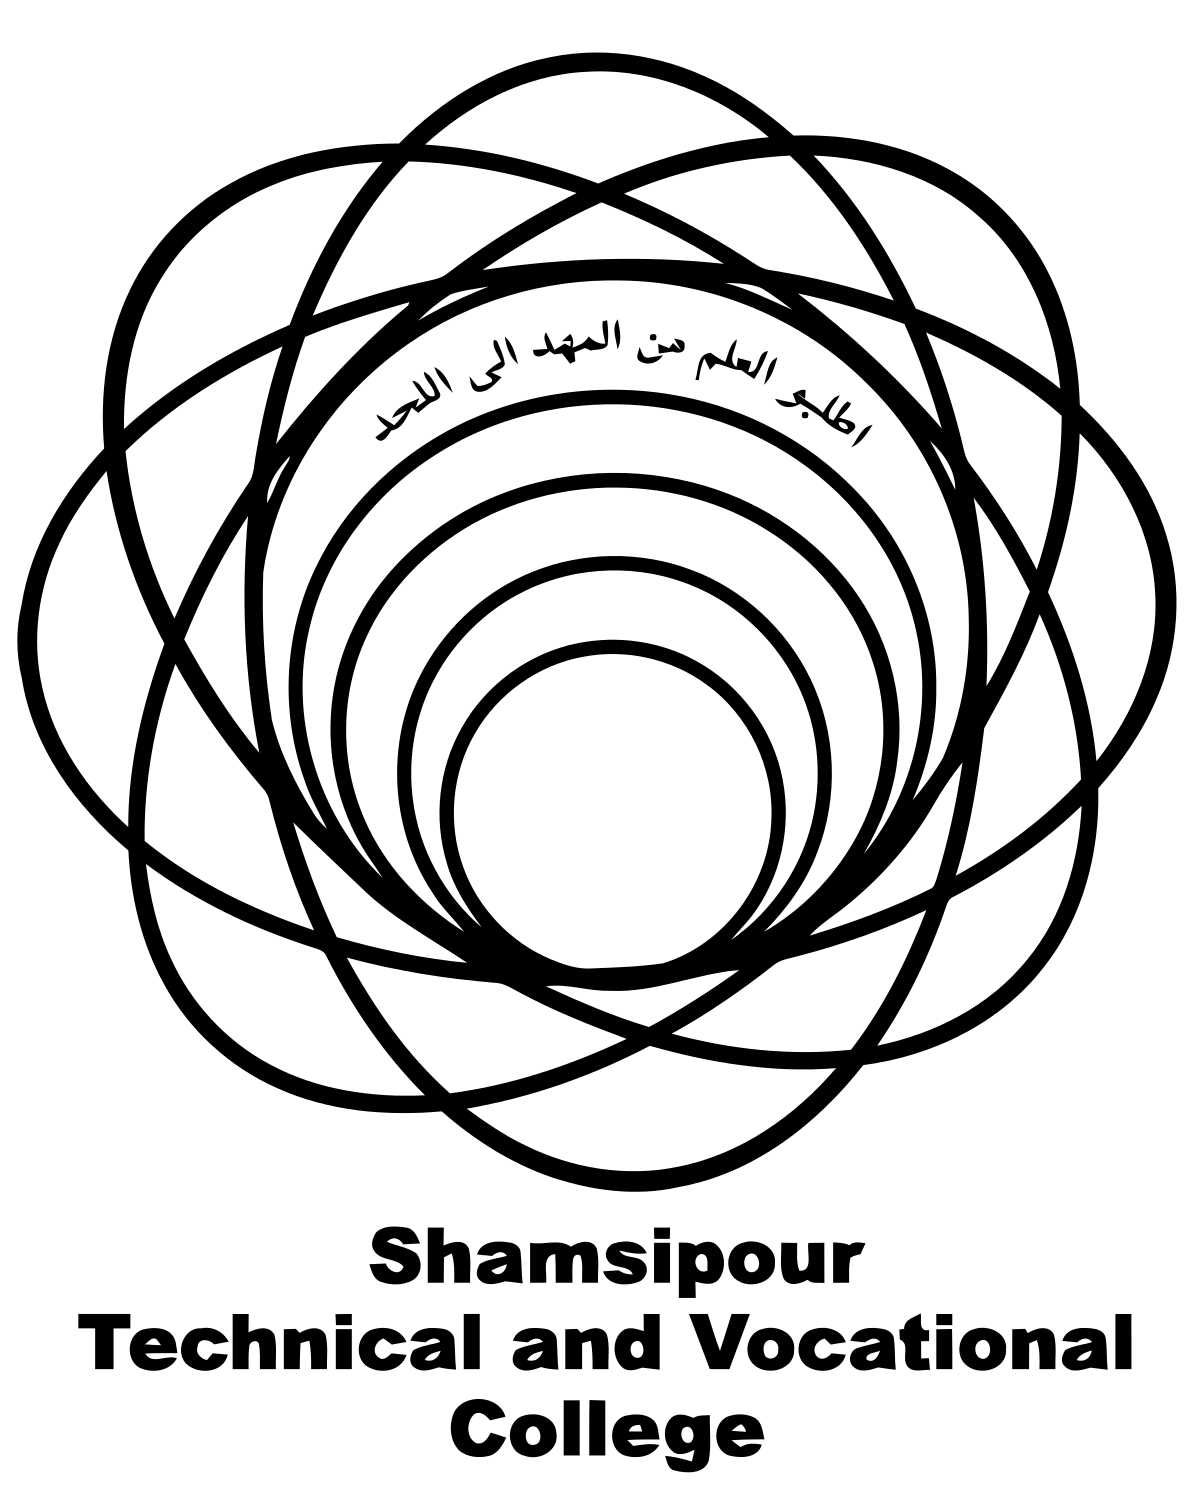
\includegraphics[width=4cm]{shamsi.png}
      \\
      \thetitle{آبیاری خودکار گلدان‌ها}
      \lesson{مباحث ویژه}
        \by{مهدی صفریان}
        \teacher{ساسان برهلیا}
        \vfill

        \uni{دانشکده فنی حرفه‌ای شهید شمسی پور}
        \thedate[\today]
    \end{center}
\end{titlepage}

\tableofcontents
\begin{titlingpage}
\title{آبیاری خودکار گلدان‌ها}
\author{مهدی صفریان}
\date{}
  \maketitle
  \begin{abstract}
   
    در این پروژه سعی شده تا با استفاده از بردهای کامپیوتری کوچک و حسگرها آبیاری گلدان‌ها را اتوماتیک کرده
    و روند آب‌ رسانی به گیاهان را مرتب و با توجه رطوبت خاک و کمبود آب در خاک مدیریت کنیم.
   
  \end{abstract}
\end{titlingpage}

%فارسی%
\section{تجهیزات}
\subsection{برد رزبری پای ۳ }
\subsection{رله}
\subsection{حسگر رطوبت}
\subsection{کابل جامپر}
\subsection{ادابتور}
\subsection{پمپ آب}

\subsection{کابل مبدل TTL به USB}
  \section{نحوه کار}

\end{document}
